\chapter{Эксперимент 1}
\section*{Добавление модели полупроводникового диода, описанного в формате \textit{PCPICE}, в базу данных \textit{MULTISIM}}

\begin{enumerate}
	\item Я создал новое семейство компонентов в \textit{User Database} и назвал его \textit{lab3}.
	\begin{figure}[H]
		\centering
		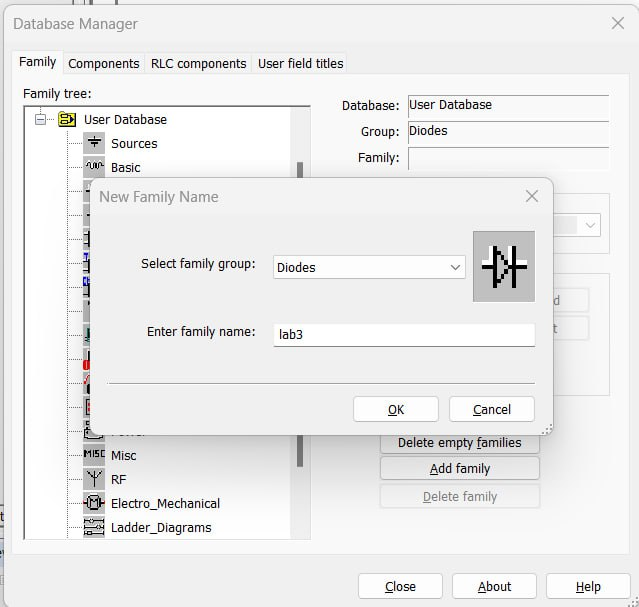
\includegraphics[width=0.65\textwidth]{img/01.jpg}
	\end{figure}
	\item Задал схемное обозначение элемента в окне \textit{Component RefDes} как \textit{D}.
	\begin{figure}[H]
		\centering
		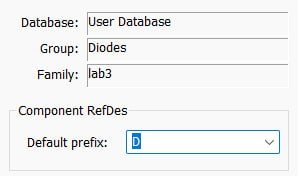
\includegraphics[width=0.65\textwidth]{img/02.jpg}
	\end{figure}
	\newpage
	\item Запустил мастер создания компонентов (\textit{Component Wizard}).
	\begin{figure}[H]
		\centering
		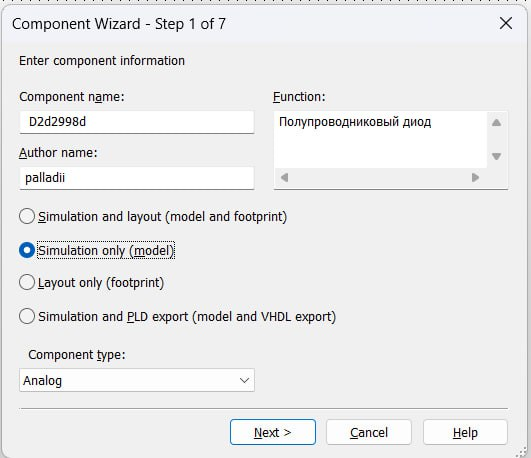
\includegraphics[width=0.6\textwidth]{img/03.jpg}
	\end{figure}
	\begin{figure}[H]
		\centering
		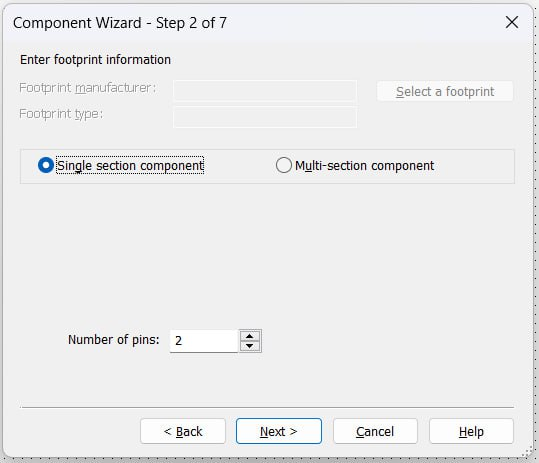
\includegraphics[width=0.6\textwidth]{img/04.jpg}
	\end{figure}
	\newpage
	\item Настроил графическое представление компонента.
	\begin{figure}[H]
		\centering
		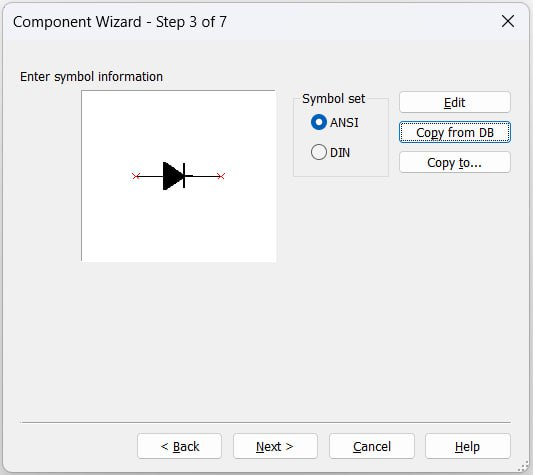
\includegraphics[width=0.6\textwidth]{img/05.jpg}
	\end{figure}
	\item Определил параметры выводов компонента.
	\begin{figure}[H]
		\centering
		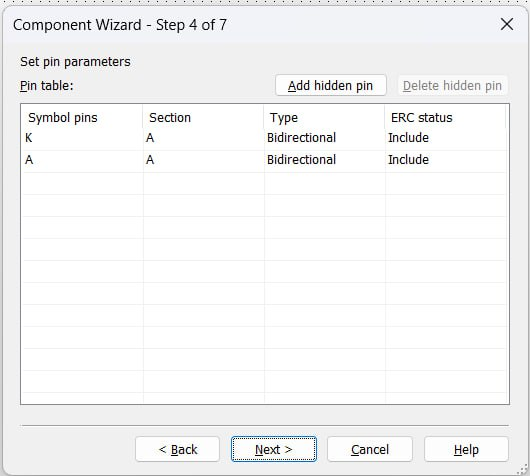
\includegraphics[width=0.6\textwidth]{img/06.jpg}
	\end{figure}
	\newpage
	\item Загрузил данные для своего диода \texttt{D2d2998d}.
	\begin{figure}[H]
		\centering
		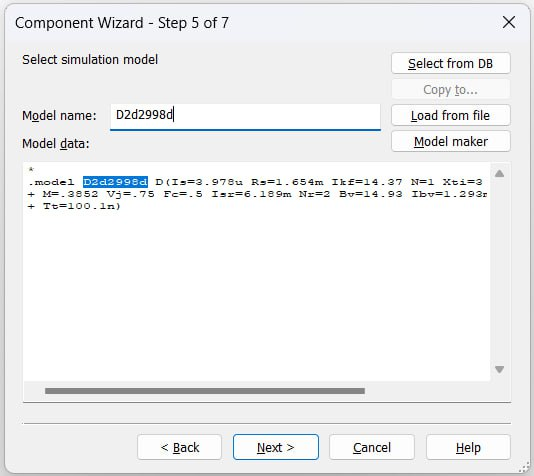
\includegraphics[width=0.6\textwidth]{img/07.jpg}
	\end{figure}
	\item Связал символ на схеме с электрической моделью, поменяв местами контакты A и K.
	\begin{figure}[H]
		\centering
		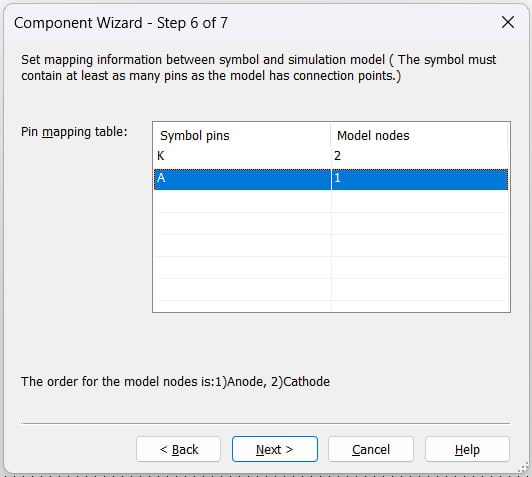
\includegraphics[width=0.6\textwidth]{img/08.jpg}
	\end{figure}
	\newpage
	\item Добавил готовый компонент в библиотеку \textit{Multisim}.
	\begin{figure}[H]
		\centering
		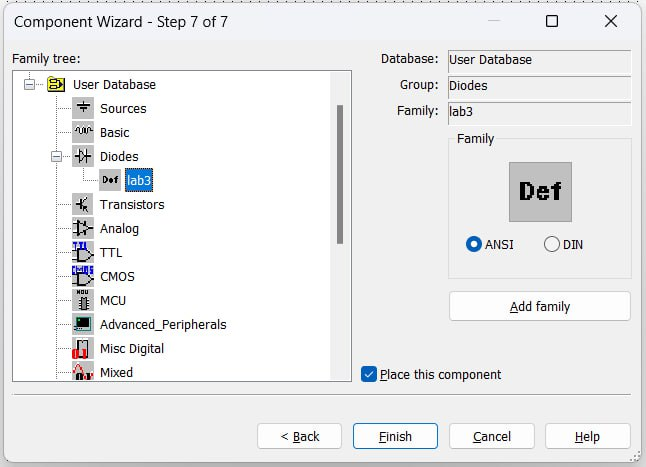
\includegraphics[width=0.6\textwidth]{img/09.jpg}
	\end{figure}
	\item Проверил, что диод появился в базе данных.
	\begin{figure}[H]
		\centering
		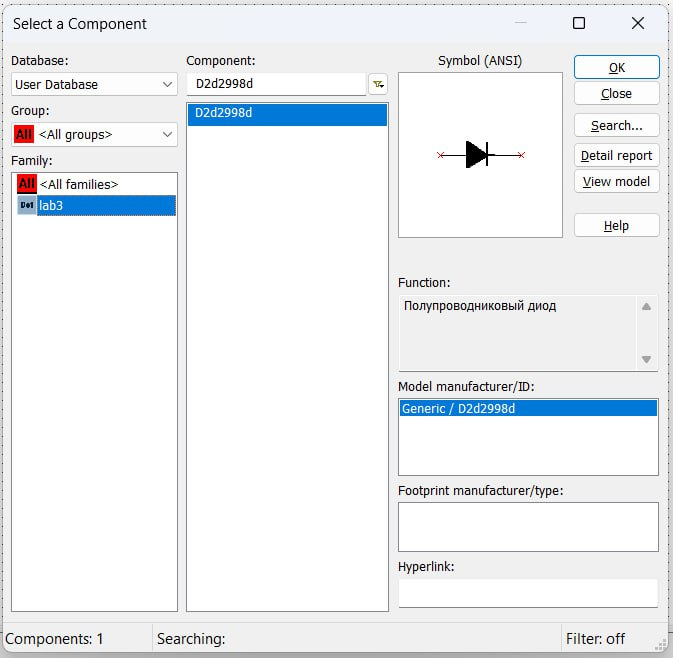
\includegraphics[width=0.6\textwidth]{img/10.jpg}
	\end{figure}
\end{enumerate}
